\documentclass[a4paper,12pt]{report}
\usepackage[utf8]{inputenc}


\usepackage{tikz}
\usetikzlibrary{calc}
\usepackage{subcaption}

\begin{document}

\thispagestyle{empty}

\begin{figure}
		\centering
		\begin{subfigure}{0.31\textwidth}
		\centering
		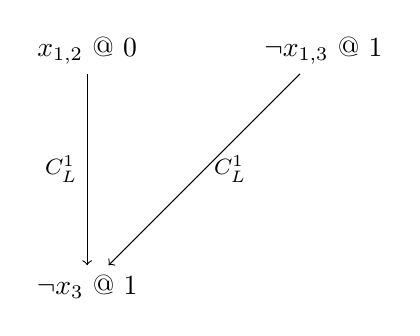
\begin{tikzpicture}[level distance=3cm]
		\node (1) {$x_{1,2}$ @ 0}
		child {node (2) {$\lnot x_3$ @ 1}
		}
		node (3) at ($(1) + (0:3cm)$) {$\lnot x_{1,3}$ @ 1}
		;
		\draw [->] (1) --  node [left] {\footnotesize{$C_L^1$}} (2) ;
		\draw [->] (3) --  node [right] {\footnotesize{$C_L^1$}} (2) ;
		\end{tikzpicture}
		\caption{}
		\end{subfigure}%
		\hfill
		\begin{subfigure}{0.31\textwidth}
		\centering
		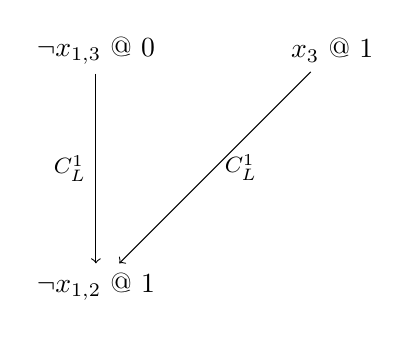
\begin{tikzpicture}[level distance=3cm]
		\node (1) {$\lnot x_{1,3}$ @ 0}
		child {node (2) {$\lnot x_{1,2}$ @ 1}
		}
		node (3) at ($(1) + (0:3cm)$) {$x_{3}$ @ 1}
		;
		\draw [->] (1) --  node [left] {\footnotesize{$C_L^1$}} (2) ;
		\draw [->] (3) --  node [right] {\footnotesize{$C_L^1$}} (2) ;
		\end{tikzpicture}
		\caption{}
		\end{subfigure}%
		\hfill
		\begin{subfigure}{0.31\textwidth}
		\centering
		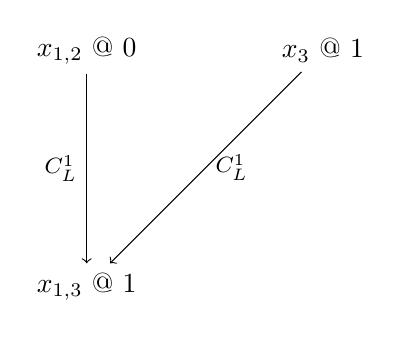
\begin{tikzpicture}[level distance=3cm]
		\node (1) {$x_{1,2}$ @ 0}
		child {node (2) {$x_{1,3}$ @ 1}
		}
		node (3) at ($(1) + (0:3cm)$) {$x_{3}$ @ 1}
		;
		\draw [->] (1) --  node [left] {\footnotesize{$C_L^1$}} (2) ;
		\draw [->] (3) --  node [right] {\footnotesize{$C_L^1$}} (2) ;
		\end{tikzpicture}
		\caption{}
		\end{subfigure}
		\caption{Implication graphs for the three cases where $C_L^1$ is used to imply a variable.}
		\label{fig:C_L_1_implication_graphs}
	\end{figure}

\end{document}
